\documentclass[11pt]{article}
\usepackage{tikz}
\usepackage{amssymb}
\usepackage{geometry}
\geometry{letterpaper, landscape, margin=0.4in}
\usetikzlibrary{positioning, calc}

% Door macros
\newcommand{\hdoor}[2]{%
  \fill[white,draw=black,thick] ({#1-0.1},{#2-0.12}) rectangle ({#1+0.1},{#2+0.12});%
}
\newcommand{\vdoor}[2]{%
  \fill[white,draw=black,thick] ({#1-0.12},{#2-0.1}) rectangle ({#1+0.12},{#2+0.1});%
}

\begin{document}

\begin{center}
{\Huge \textbf{The Grain Mother's Ruin}}\\[0.3em]
{\Large Level 3A --- The Deep Sanctum | 12 Keyed Areas}
\end{center}

\vspace{0.3em}

\begin{center}
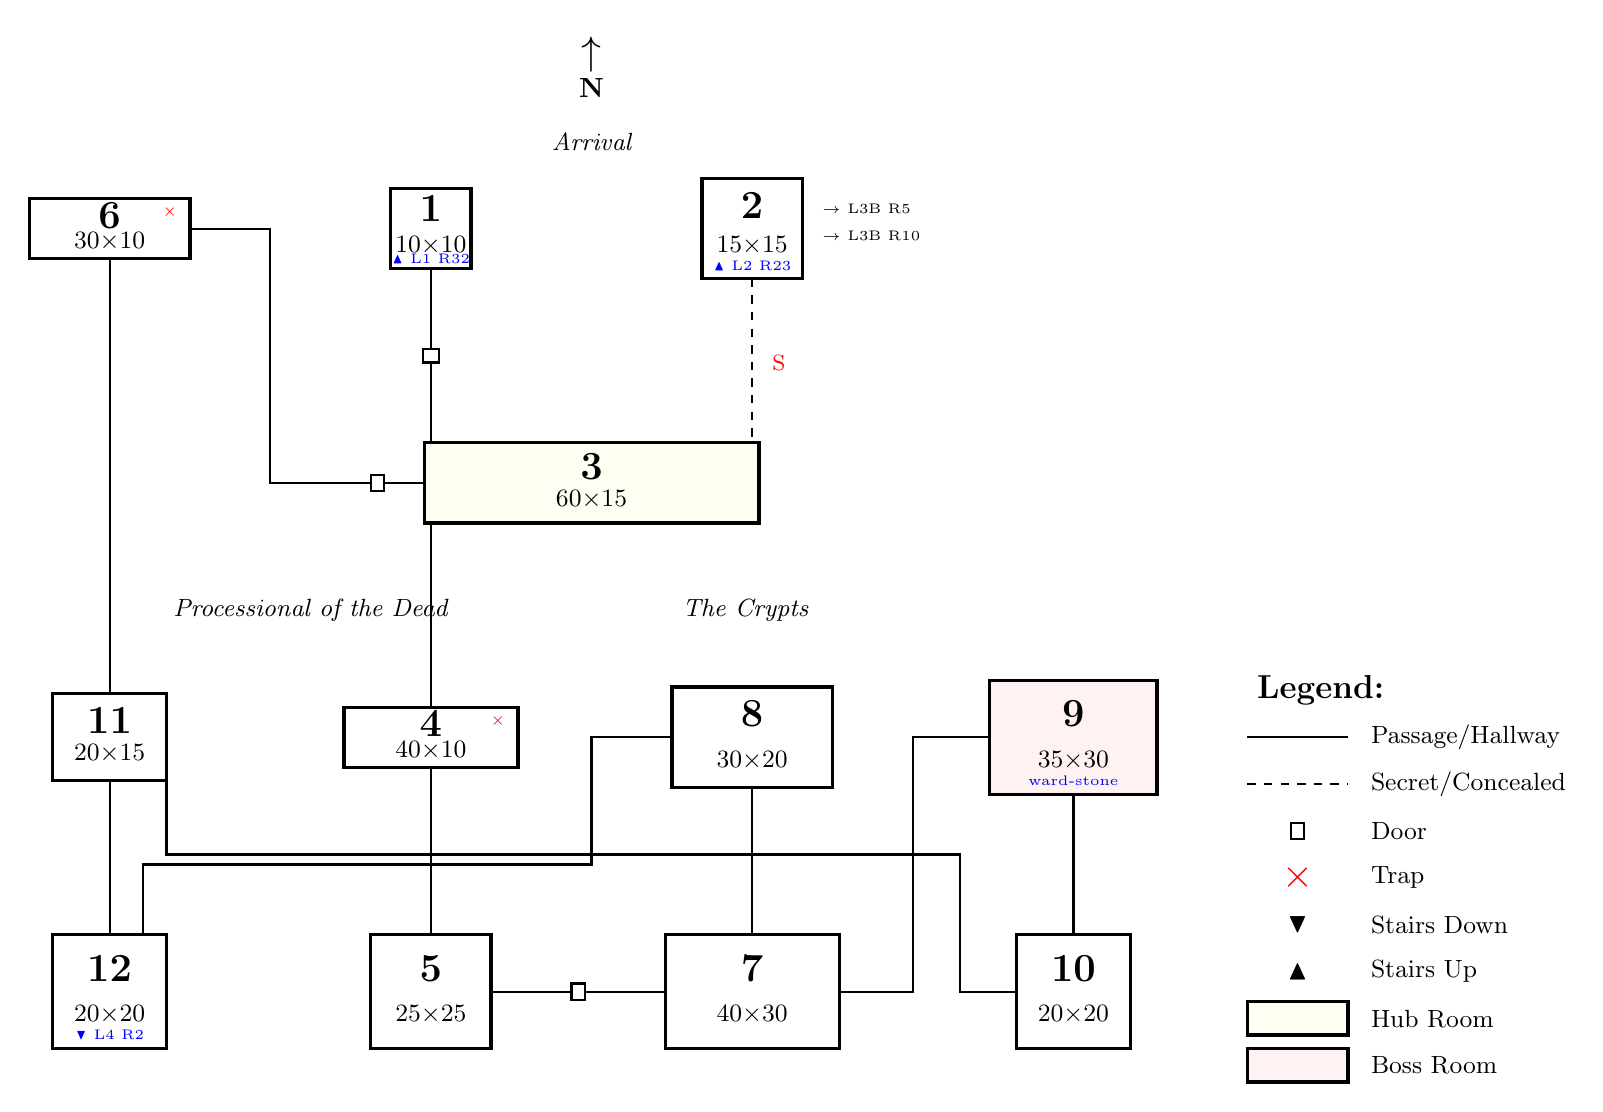
\begin{tikzpicture}[
    room/.style={draw, very thick, rectangle},
    hub/.style={draw, very thick, rectangle, fill=yellow!5},
    boss/.style={draw, very thick, rectangle, fill=red!5},
    connection/.style={draw, thick},
    secret/.style={dashed, thick},
    trap/.style={red},
    scale=0.85
]

% ============================================================
% GRID PARAMETERS
% CellW=3.0, CellH=2.0, Gutter=1.8
% Cols: c0(x=1.5) c1(x=6.3) c2(x=11.1) c3(x=15.9)
% Rows: r0(y=1.0) r1(y=4.8) r2(y=8.6) r3(y=12.4)
% Vertical gutters: c0-c1(x=3.9) c1-c2(x=8.7) c2-c3(x=13.5)
% Horizontal gutters: r0-r1(y=2.9) r1-r2(y=6.7) r2-r3(y=10.5)
% ============================================================

% ============================================================
% NORTH ARROW
% ============================================================
\node at (8.7, 15.0) {\Large $\uparrow$};
\node at (8.7, 14.5) {\textbf{N}};

% ============================================================
% ZONE: Arrival (Rooms 1-2)
% Grid region: r3
% ============================================================

% Room 1: The Warded Landing (10x10 ft)
% Cell: (c1, r3) -> center (6.3, 12.4)
% Rect: (5.7, 11.8) to (6.9, 13.0)
\draw[room] (5.7,11.8) rectangle (6.9,13.0);
\node at (6.3,12.7) {\Large \textbf{1}};
\node[font=\small] at (6.3,12.15) {10$\times$10};
\node[blue,font=\tiny] at (6.3,11.95) {$\blacktriangle$ L1 R32};

% Room 2: The Pilgrim's Stair (15x15 ft)
% Cell: (c2, r3) -> center (11.1, 12.4)
% Rect: (10.35, 11.65) to (11.85, 13.15)
\draw[room] (10.35,11.65) rectangle (11.85,13.15);
\node at (11.1,12.75) {\Large \textbf{2}};
\node[font=\small] at (11.1,12.15) {15$\times$15};
\node[blue,font=\tiny] at (11.1,11.85) {$\blacktriangle$ L2 R23};

% Level 3B connection annotations for Room 2
\node[font=\tiny,anchor=west] at (12.0,12.7) {$\rightarrow$ L3B R5};
\node[font=\tiny,anchor=west] at (12.0,12.3) {$\rightarrow$ L3B R10};

% ============================================================
% ZONE: The Processional of the Dead (Rooms 3-6)
% Grid region: r2-r3 (R6), r2 (R3), r1-r0 (R4-R5)
% ============================================================

% Room 3: The Hall of Remembrance (60x15 ft)
% Cell: (c1-c2, r2) -> center (8.7, 8.6), spans 2 cells
% Rect: (6.2, 8.0) to (11.2, 9.2)
\draw[hub] (6.2,8.0) rectangle (11.2,9.2);
\node at (8.7,8.85) {\Large \textbf{3}};
\node[font=\small] at (8.7,8.35) {60$\times$15};

% Room 4: The Corridor of Trials (40x10 ft)
% Cell: (c1, r1) -> center (6.3, 4.8)
% Rect: (5.0, 4.35) to (7.6, 5.25)
\draw[room] (5.0,4.35) rectangle (7.6,5.25);
\node at (6.3,5.0) {\Large \textbf{4}};
\node[font=\small] at (6.3,4.6) {40$\times$10};
\node[red,font=\tiny] at (7.3,5.05) {$\times$};

% Room 5: The Antechamber of Judgement (25x25 ft)
% Cell: (c1, r0) -> center (6.3, 1.0)
% Rect: (5.4, 0.15) to (7.2, 1.85)
\draw[room] (5.4,0.15) rectangle (7.2,1.85);
\node at (6.3,1.35) {\Large \textbf{5}};
\node[font=\small] at (6.3,0.65) {25$\times$25};

% Room 6: The Offering Alcoves (30x10 ft)
% Cell: (c0, r3) -> center (1.5, 12.4)
% Rect: (0.3, 11.95) to (2.7, 12.85)
\draw[room] (0.3,11.95) rectangle (2.7,12.85);
\node at (1.5,12.6) {\Large \textbf{6}};
\node[font=\small] at (1.5,12.2) {30$\times$10};
\node[red,font=\tiny] at (2.4,12.65) {$\times$};

% ============================================================
% ZONE: The Crypts (Rooms 7-12)
% Grid region: r0-r1
% ============================================================

% Room 7: The Warriors' Crypt (40x30 ft)
% Cell: (c2, r0) -> center (11.1, 1.0)
% Rect: (9.8, 0.15) to (12.4, 1.85)
\draw[room] (9.8,0.15) rectangle (12.4,1.85);
\node at (11.1,1.35) {\Large \textbf{7}};
\node[font=\small] at (11.1,0.65) {40$\times$30};

% Room 8: The Acolytes' Ossuary (30x20 ft)
% Cell: (c2, r1) -> center (11.1, 4.8)
% Rect: (9.9, 4.05) to (12.3, 5.55)
\draw[room] (9.9,4.05) rectangle (12.3,5.55);
\node at (11.1,5.15) {\Large \textbf{8}};
\node[font=\small] at (11.1,4.45) {30$\times$20};

% Room 9: The High Priests' Tombs (35x30 ft) -- BOSS: Mummy + Ward-Stone
% Cell: (c3, r1) -> center (15.9, 4.8)
% Rect: (14.65, 3.95) to (17.15, 5.65)
\draw[boss] (14.65,3.95) rectangle (17.15,5.65);
\node at (15.9,5.15) {\Large \textbf{9}};
\node[font=\small] at (15.9,4.45) {35$\times$30};
\node[blue,font=\tiny] at (15.9,4.15) {ward-stone};

% Room 10: The Tomb of Archon Theron (20x20 ft)
% Cell: (c3, r0) -> center (15.9, 1.0)
% Rect: (15.05, 0.15) to (16.75, 1.85)
\draw[room] (15.05,0.15) rectangle (16.75,1.85);
\node at (15.9,1.35) {\Large \textbf{10}};
\node[font=\small] at (15.9,0.65) {20$\times$20};

% Room 11: The Reliquary of the Faithful (20x15 ft)
% Cell: (c0, r1) -> center (1.5, 4.8)
% Rect: (0.65, 4.15) to (2.35, 5.45)
\draw[room] (0.65,4.15) rectangle (2.35,5.45);
\node at (1.5,5.05) {\Large \textbf{11}};
\node[font=\small] at (1.5,4.55) {20$\times$15};

% Room 12: The Preparation Chamber (20x20 ft)
% Cell: (c0, r0) -> center (1.5, 1.0)
% Rect: (0.65, 0.15) to (2.35, 1.85)
\draw[room] (0.65,0.15) rectangle (2.35,1.85);
\node at (1.5,1.35) {\Large \textbf{12}};
\node[font=\small] at (1.5,0.65) {20$\times$20};
\node[blue,font=\tiny] at (1.5,0.35) {$\blacktriangledown$ L4 R2};

% ============================================================
% CONNECTIONS
% ============================================================

% Room 1 -> Room 3 (door, stone door)
% Route: vertical from R1 bottom to R3 top, through gutter r2-r3
\draw[thick] (6.3,11.8) -- (6.3,9.2);
\vdoor{6.3}{10.5}

% Room 2 -> Room 3 (concealed panel, secret-style)
% Route: vertical from R2 bottom to R3 top-right
\draw[thick,dashed] (11.1,11.65) -- (11.1,9.2);
\node[red,font=\footnotesize] at (11.5,10.4) {S};

% Room 3 -> Room 4 (open corridor)
% Route: vertical from R3 bottom-left to R4 top, through gutter r1-r2
\draw[thick] (6.3,8.0) -- (6.3,5.25);

% Room 3 -> Room 6 (door)
% Route: L-shape from R3 left edge, through gutter c0-c1 to R6 right edge
\draw[thick] (6.2,8.6) -- (3.9,8.6) -- (3.9,12.4) -- (2.7,12.4);
\hdoor{5.5}{8.6}

% Room 4 -> Room 5 (open corridor)
% Route: vertical from R4 bottom to R5 top, through gutter r0-r1
\draw[thick] (6.3,4.35) -- (6.3,1.85);

% Room 5 -> Room 7 (door, puzzle stone slab)
% Route: horizontal from R5 right to R7 left, through gutter c1-c2
\draw[thick] (7.2,1.0) -- (9.8,1.0);
\hdoor{8.5}{1.0}

% Room 6 -> Room 11 (open passage)
% Route: vertical from R6 bottom to R11 top, through gutters r2-r3 and r1-r2
\draw[thick] (1.5,11.95) -- (1.5,5.45);

% Room 7 -> Room 8 (open passage)
% Route: vertical from R7 top to R8 bottom, through gutter r0-r1
\draw[thick] (11.1,1.85) -- (11.1,4.05);

% Room 7 -> Room 9 (open passage)
% Route: L-shape from R7 right edge, through gutter c2-c3, to R9 left edge
\draw[thick] (12.4,1.0) -- (13.5,1.0) -- (13.5,4.8) -- (14.65,4.8);

% Room 8 -> Room 12 (open passage, west of R8)
% Route: from R8 left edge, through gutter c1-c2, south through gutter r0-r1, west to R12
\draw[thick] (9.9,4.8) -- (8.7,4.8) -- (8.7,2.9) -- (2.0,2.9) -- (2.0,1.85);

% Room 9 -> Room 10 (open passage)
% Route: vertical from R9 bottom to R10 top, through gutter r0-r1
\draw[thick] (15.9,3.95) -- (15.9,1.85);

% Room 10 -> Room 11 (open passage, west of R10)
% Route: from R10 left edge, through gutter c2-c3, west through gutter r0-r1, to R11 right edge
\draw[thick] (15.05,1.0) -- (14.2,1.0) -- (14.2,3.05) -- (2.35,3.05) -- (2.35,4.8);

% Room 11 -> Room 12 (open passage)
% Route: vertical from R11 bottom to R12 top, through gutter r0-r1
\draw[thick] (1.5,4.15) -- (1.5,1.85);

% ============================================================
% LEGEND
% ============================================================
\node[anchor=west,font=\large] at (18.5,5.5) {\textbf{Legend:}};

\draw[thick] (18.5,4.8) -- (20.0,4.8);
\node[anchor=west,font=\small] at (20.2,4.8) {Passage/Hallway};

\draw[thick,dashed] (18.5,4.1) -- (20.0,4.1);
\node[anchor=west,font=\small] at (20.2,4.1) {Secret/Concealed};

\fill[white,draw=black,thick] (19.15,3.28) rectangle (19.35,3.52);
\node[anchor=west,font=\small] at (20.2,3.4) {Door};

\node[red] at (19.25,2.7) {\Large $\times$};
\node[anchor=west,font=\small] at (20.2,2.7) {Trap};

\node at (19.25,2.0) {$\blacktriangledown$};
\node[anchor=west,font=\small] at (20.2,2.0) {Stairs Down};

\node at (19.25,1.3) {$\blacktriangle$};
\node[anchor=west,font=\small] at (20.2,1.3) {Stairs Up};

\draw[yellow!5,very thick] (18.5,0.6) rectangle (20.0,0.6);
\draw[very thick,fill=yellow!5] (18.5,0.35) rectangle (20.0,0.85);
\node[anchor=west,font=\small] at (20.2,0.6) {Hub Room};

\draw[very thick,fill=red!5] (18.5,-0.35) rectangle (20.0,0.15);
\node[anchor=west,font=\small] at (20.2,-0.1) {Boss Room};

% ============================================================
% ZONE LABELS
% ============================================================
\node[font=\small\itshape] at (8.7,13.7) {Arrival};
\node[font=\small\itshape] at (4.5,6.7) {Processional of the Dead};
\node[font=\small\itshape] at (11.0,6.7) {The Crypts};

\end{tikzpicture}
\end{center}

\vspace{0.5em}

% ============================================================
% ROOM KEY TABLE
% ============================================================
\section*{Room Key}
\begin{small}
\begin{tabular}{rl|rl|rl}
1 & Warded Landing (10$\times$10) & 5 & Antechamber of Judgement (25$\times$25) & 9 & High Priests' Tombs (35$\times$30) \\
2 & Pilgrim's Stair (15$\times$15) & 6 & Offering Alcoves (30$\times$10) & 10 & Tomb of Archon Theron (20$\times$20) \\
3 & Hall of Remembrance (60$\times$15) & 7 & Warriors' Crypt (40$\times$30) & 11 & Reliquary of the Faithful (20$\times$15) \\
4 & Corridor of Trials (40$\times$10) & 8 & Acolytes' Ossuary (30$\times$20) & 12 & Preparation Chamber (20$\times$20) \\
\end{tabular}
\end{small}

% ============================================================
% INTER-LEVEL CONNECTIONS
% ============================================================
\section*{Connections to Other Levels}
\begin{small}
\begin{itemize}
    \item \textbf{Room 1 (Warded Landing):} Spiral staircase up to Level 1, Room 32 (The Sealed Shrine)
    \item \textbf{Room 2 (Pilgrim's Stair):} Hidden spiral staircase up to Level 2, Room 23 (Hidden Descent)
    \item \textbf{Room 2 (Pilgrim's Stair):} Worm breach east to Level 3B, Room 5 (Acid-Bored Tunnel)
    \item \textbf{Room 2 (Pilgrim's Stair):} Concealed door south to Level 3B, Room 10 (Passage to the Sanctum)
    \item \textbf{Room 12 (Preparation Chamber):} Secret warded staircase down to Level 4, Room 2 (Priest's Landing)
\end{itemize}
\end{small}

\end{document}
